\section{Dynamic Scheduler Results Under Fixed and Variable Load}
\label{sec:dynamicresults}
% Double-column floats are defined here so that they appear on the page where R1/R2 are discussed
% (LaTeX keeps single- and double-column floats in sequence).
\begin{table*}[t]
\centering\footnotesize
\caption{R1 fixed-rate physical results; means over ten paired blocks. Adjusted power subtracts the immediately preceding idle. Escalation is the fraction sent from LightLR to MedRF.}
\label{tab:r1}
\setlength{\tabcolsep}{4.0pt}
\begin{tabular}{lrrrrrrr}\toprule
Method & Energy (J) & Power (W) & Adjusted (mW) & F1 & Recall (\%) & FPR (\%) & Escalation (\%)\\\midrule
\tableinput{tables/r1_revision_rows}
\bottomrule\end{tabular}
\end{table*}

\begin{table*}[t]
\centering\footnotesize
\caption{Corrected R2 over ten paired blocks. Energy is mean$\pm$SD across runs; miss is the fraction of one-second windows missing deadline. Completion p95 is the mean of within-run 95th-percentile window completion times.}
\label{tab:r2}
\setlength{\tabcolsep}{3.1pt}
\begin{tabular}{lrrrrrrr}\toprule
Method & Energy (J) & Power (W) & F1 & Recall (\%) & FPR (\%) & Miss (\%) & Completion p95 (s)\\\midrule
\tableinput{tables/r2_revision_rows}
\bottomrule\end{tabular}
\end{table*}

\begin{figure*}[!t]
\centering
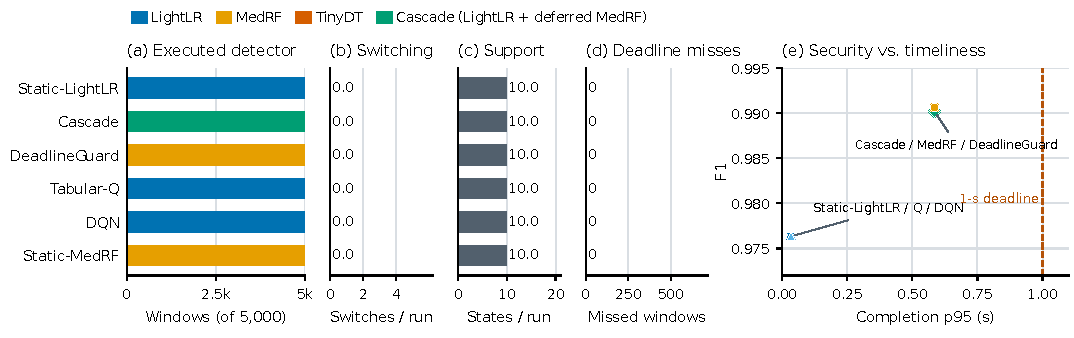
\includegraphics[width=\textwidth]{figures/r2_operational_dashboard.pdf}
\caption{Corrected R2 operational summary across 60 runs: (a) executed paths; (b) runtime action changes, excluding initialization; (c) unique 108-state indices per run; (d) deadline misses; (e) F1 versus mean run-level completion p95, with the 1-s deadline dashed. Q/DQN stay LightLR, DeadlineGuard stays MedRF, and all methods have zero recorded misses. Cascade denotes a conditional LightLR-plus-MedRF path, not a single-detector action.}
\label{fig:r2dashboard}
\end{figure*}

This section retains the fixed-rate R1 campaign and reports the corrected variable-load R2 comparison separately from historical variable-load execution. R1 uses its original fixed-load policies; corrected R2 uses the 108-state service-penalized setting in Section~\ref{sec:methods}. R3 remains a protocol-preserving stop and R4 a validation-only threshold diagnostic. No historical and corrected measurements are pooled.

\subsection{R1: Fixed-Rate Confidence Cascade}
Table~\ref{tab:r1} reports ten new matched blocks at 100 rows/s. The fixed cascade escalates 1.34\% of rows and raises F1 by 1.347~pp over Static-LightLR while spending +7.952~J with 95\% CI $[5.897,\,10.007]$~J. Its raw mean-power difference is +15.917~mW $[11.798,\,20.035]$, whereas the preceding-idle adjustment gives +13.635~mW $[-1.515,\,28.784]$: environmental drift therefore weakens the power attribution but not the raw-energy result. Cascade F1 (0.98391) matches Static-MedRF (0.98386) within a few $10^{-5}$, at 0.279~pp lower recall and 0.156~pp lower FPR.

\subsubsection*{Cascade cost is a call-granularity phenomenon, not a bound}
The apparently disproportionate cascade latency at a 1.34\% escalation rate is explained by call granularity. The frozen source performs \emph{one} MedRF call per escalation-active window on the deferred sub-batch, not one MedRF call per deferred row. Although only 1.3388\% of the 500{,}000 rows are deferred, they land in 3{,}338 of 5{,}000 windows (66.76\%), with a mean of only 2.01 deferred rows per active window. No-escalation windows average 1.636~ms; any-escalation windows average 31.884~ms, close to the cost of a single MedRF batch call regardless of sub-batch size; the overall mean is 21.830~ms. This is an operating-point description, not a general bound: an optimized batched cascade with wider windows or amortized MedRF calls would show a different profile. What the measurement establishes is that reporting only the escalation \emph{fraction} would be misleading; escalation \emph{prevalence across windows} is the operational cost driver.

\subsection{R2: Variable-Load Factorial and DeadlineGuard}
Each corrected R2 run visits the nine fixed load-by-prevalence cells for 50 windows each, followed by 50 recovery windows. All methods receive the same workload within block; no cell identity or label is an online feature. The learned controllers and DeadlineGuard share current arrivals and pre-append carryover; Cascade additionally observes current-row confidence after entry inference. Table~\ref{tab:r2} gives all six means and Table~\ref{tab:r2pairs} gives matched-static and cascade contrasts.

\begin{table}[t]
\centering\footnotesize
\caption{Headline R2 paired contrasts ($n=10$ blocks). Differences are first-minus-second method; F1 and deadline-miss changes are percentage points.}
\label{tab:r2pairs}
\setlength{\tabcolsep}{5pt}
\resizebox{\columnwidth}{!}{%
\begin{tabular}{lrrr}\toprule
 & Cascade $-$ & Q $-$ & DQN $-$\\
Endpoint & Static-MedRF & Static-LightLR & Static-LightLR\\\midrule
\tableinput{tables/r2_key_paired_rows}
\bottomrule\end{tabular}}
\end{table}

\subsubsection*{DeadlineGuard: no realized load-conditioned switching}
DeadlineGuard executes MedRF in all 5{,}000 windows, as does Static-MedRF; both have identical within-block detection summaries and zero recorded misses. Its calibrated demand test never triggers LightLR on these traces. Static-LightLR, Q, DQN and Cascade also record zero misses. Hence the corrected experiment does not demonstrate deadline-violation removal, load-triggered switching gains or a superiority claim for DeadlineGuard. The historical 43.7-J/512-miss result arose under a different execution interface and is not a corrected-R2 result.

Cascade minus Static-MedRF has mean energy difference $-12.064$~J, paired 95\% CI $[-16.548,-7.580]$~J. F1 changes by $-0.0004457$ ($-0.0446$~pp), recall by $-0.2411$~pp, and FPR by $-0.1534$~pp. Lower FPR thus accompanies lower recall and F1, not a cost-free improvement. This variable-load trade-off is implementation-specific; it is not the historical 1.373-pp DeadlineGuard comparison or the fixed-rate R1 call-cost regime.

\subsubsection*{Learned selectors and matched static controls}
Corrected Q and DQN each select LightLR in every one of their 5{,}000 windows and reproduce Static-LightLR detection exactly. Their mean energy differences from Static-LightLR are respectively +0.246~J $[-4.055,4.547]$~J and +0.599~J $[-4.119,5.317]$~J. Neither interval resolves an energy benefit; neither proves equivalence. The historical Tabular-Q TinyDT trajectory used mismatched load timing and post-append queue normalization and is retained as an implementation diagnostic, not evidence that the corrected common-interface policy fails on new load bins. The original 314/324 map remains specific to its original fixed-load policy.

\subsubsection*{Interrupted blocks and preceding-idle sensitivity}
Block 1 retains five accepted methods plus a newly numbered Static-LightLR replacement after external CPU rejection; block 5 retains its accepted runs and replaces the failed Cascade idle before its first formal workload. Both span periods. A maintenance task coincides with the first failure; the second revealed processing overhead added to a fixed sampling wait. The monitor repair changes wait cadence and rejected-gap logging, not the 5\% CPU or 1.5-s interval limits. The old rejected right snapshot is absent, so its exact gap cannot be reconstructed. We report all-valid A, exclude-block-1 B, and exclude-blocks-1/5 C under raw and idle-adjusted endpoints (Supplementary Table~S24). Registration timing is disclosed; no favourable set is selected. Idle adjustment does not establish removal of temporal or instrumentation confounding. Figure~\ref{fig:r2dashboard} reports the corrected occupancy, service and state observations. The old DQN block-4 excursion remains a separate historical diagnostic without precise CPU-joule attribution.

\subsection{R3: Protocol-Preserving Stop}
R3 predeclared controller-only physical power over four ``original observed-support states'' for isolated attribution. The frozen artifact exposes eight such states and supplies no outcome-independent rule for selecting four. Choosing four \emph{after the fact} would allow controller-power reporting to be driven by known R2 results, so the campaign stopped before measurement per the predeclared stop rule. No controller-only joule value is claimed. Its stop remains unchanged; neither the corrected DQN--LightLR contrast nor timing is assigned a controller-only joule interpretation.

\subsection{R4: Threshold Calibration Diagnostic}
R4 selects a TinyDT threshold on validation by maximum balanced accuracy (highest-threshold tie-break), hashes it, and applies it \emph{once} to test. Table~\ref{tab:r4} contrasts the frozen primary threshold with the validation-selected diagnostic.

\begin{table}[t]
\centering\footnotesize
\caption{TON-IoT TinyDT test results at the fixed primary threshold and the post-hoc validation-selected threshold. The diagnostic does not replace the primary threshold; it isolates calibration sensitivity as an explanation for the primary failure.}
\label{tab:r4}
\setlength{\tabcolsep}{5pt}
\begin{tabular}{lrr}\toprule
Quantity & Primary (fixed) & Validation-selected\\\midrule
\tableinput{tables/r4_threshold_main_rows}
\bottomrule\end{tabular}
\end{table}

The diagnostic yields F1 0.9698, FPR 1.82\%, recall 99.61\%, BA 0.9889, and AUROC 0.9906. Recall changes by only 0.15~pp, so the primary failure at threshold 0.5 is substantially calibration-sensitive rather than a symptom of missing ranking information. Two consequences follow. First, TinyDT is not rehabilitated for the frozen physical campaigns: every classifier and scheduler artifact in those campaigns was fixed at threshold 0.5, and no post-hoc threshold can retroactively undo the historical TinyDT actions emitted under the earlier R2 interface; corrected R2 does not select TinyDT. Second, calibration governance---validation-only threshold selection with a hashed freeze before test---is a deployable practice that we recommend for any operational IDS pipeline that includes a TinyDT-class detector.
